\chapter{LaRE - Laboratório Remoto Expansível}
\label{Capítulo3}
\begin{center}
    \textit{``All we have to decide is what to do with the time that is given us.''}
     
     Gandalf
\end{center}

Neste capítulo descreve-se o processo que levou à criação do \acrshort{lare}, a arquitectura de \textit{hardware} e \textit{software}, o motivo das escolhas e a implementação dos circuitos. \textbf{Acho que tem de ser refeito ou complementado}

\section{Contextualização}
\label{sec:contextualização}
Como já foi referido anteriormente (\textbf{ver a referência}) o principal objectivo desta dissertação passa pelo desenvolvimento de um \acrshort{laboratório remoto} para o ensino da electrónica, que visa colmatar (ou resolver) alguns dos problemas presentes no \acrshort{visir}.

De facto, apesar de o \textit{software} do \acrshort{visir} ser de código aberto, (lançado sob a \acrshort{gpl}) - nomeadamente, o \acrshort{lms}, a componente gráfica do lado do cliente, Figura \ref{fig:protboard_visir} e o servidor de medições \cite{tawfikdcdc} - existe o problema da componente proprietária. Do lado do servidor, como referido na Secção \ref{sec:visir}, existe o \acrshort{labview} assim como a placa controladora \acrshort{pxi} e os respectivos módulos (instrumentos), proprietários da \acrshort{ni}. Há ainda a referir o facto de o \textit{software} de programação do \textit{firmware} do controlador da matriz que é vendido com a própria matriz ser proprietário da \acrshort{bth}.

Portanto, o desenvolvimento e criação do \acrshort{laboratório remoto} partiu destes pressupostos. Na sua fase mais embrionária, o projecto utilizaria um microcontrolador que, juntamente com um \acrfull{ide} desenvolvido em \acrshort{labview}, pudesse controlar um conjunto de relés. Foram feitos alguns testes com o \gls{arduino} Mega, mas, dada a complexidade do projecto e, também, uma grande vontade de desenvolver os conhecimentos ao nível do \textit{Python}\footnote{Falaremos um pouco mais sobre esta linguagem nos capítulos seguintes.}, decidiu-se avançar com este tipo de linguagem.

\begin{figure}[hbtp]
    \centering
    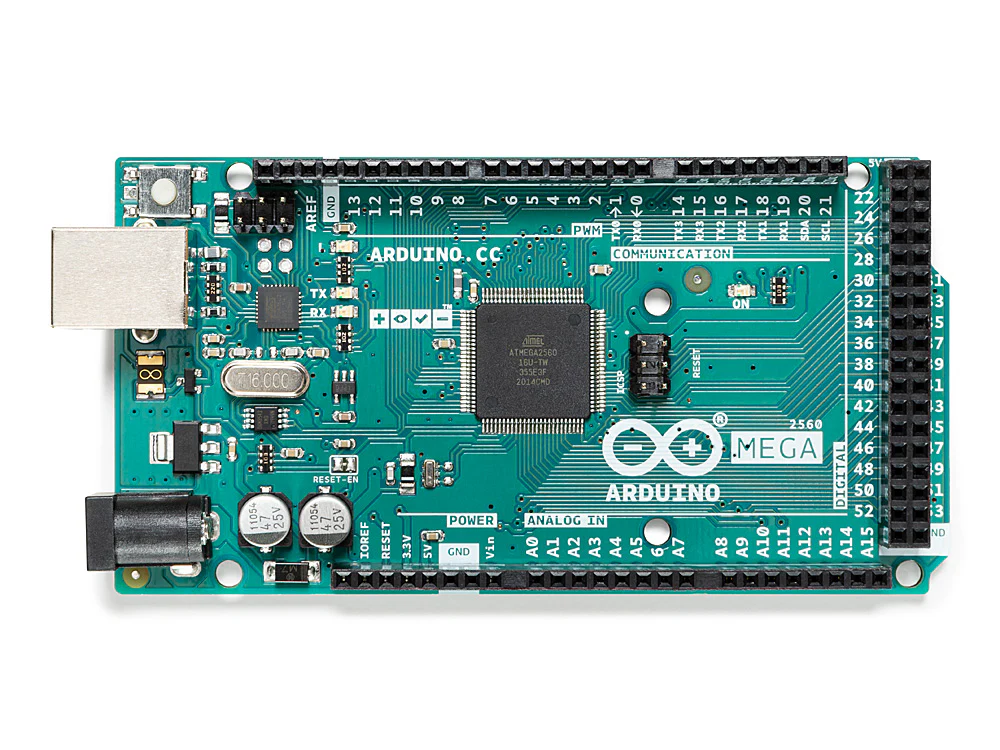
\includegraphics[width=0.6\textwidth]{figures/arduinomega.png}
    \caption{\textit{Arduino} Mega \cite{ArduinoMega}}
    \label{fig:arduinomega}
\end{figure}

É possível combinar o \textit{Arduino} com o \textit{Python}, mas isso implicaria uma mudança no \textit{firmware}. No entanto, existindo no mercado o \gls{ESP32}, muito mais poderoso decidiu-se, então, avaliar a integração do \gls{ESP32} com o \textit{Python}. Para sermos rigorosos, o uso do \textit{Python} no \gls{ESP32} faz-se através de \textit{MicroPython}, uma implementação leve da linguagem \textit{Python} especificamente projetada para microcontroladores \cite{micropythonesp32}\cite{MicroPythonlib}.
Após uma análise do \textit{datasheet} \cite{esp32datasheet}, chegou-se à conclusão de que o \gls{ESP32} com \textit{MicroPython} tem limitações de memória. De facto, a memória \textit{flash} varia entre os 4-16 \acrlong{mb}. No modelo ''ESP32-DEVKITC-32E``, que estava disponível para este projecto, era de 4 \acrshort{mb} \cite{diferencaspython}. 

\begin{figure}[hbtp]
    \centering
    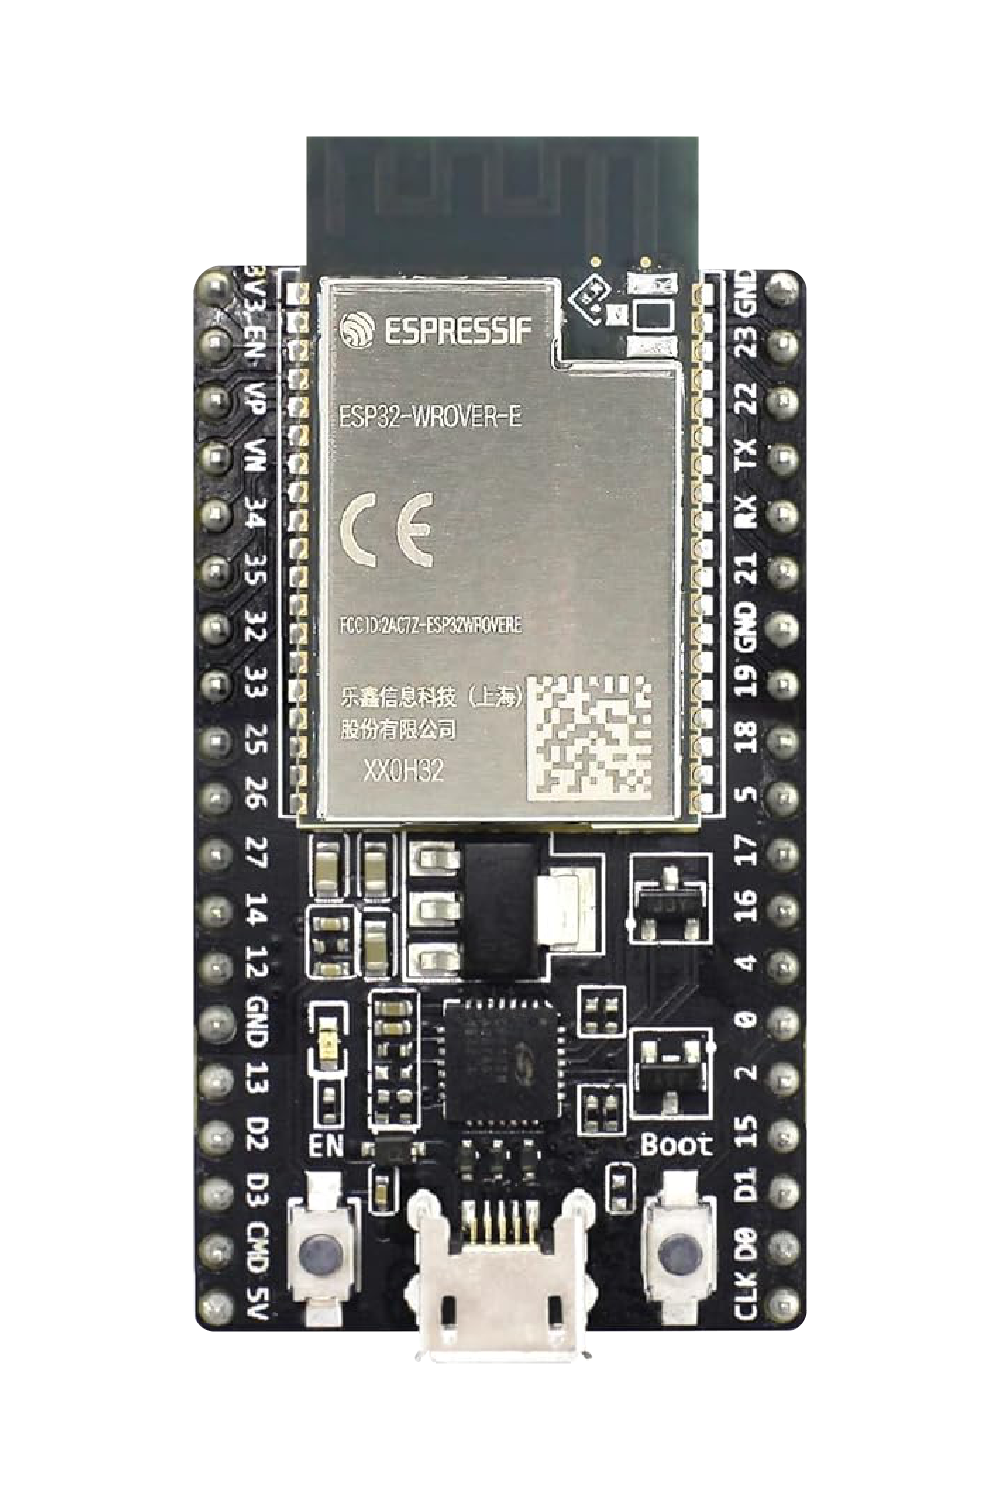
\includegraphics[width=0.4\textwidth]{figures/ESP32-DevKitC_L_0.png}
    \caption{\textit{ESP32} \cite{ESPDevKit}}
    \label{fig:ESP32}
\end{figure}

Se o objectivo era trabalhar e programar com \textit{Python}, era preciso outro tipo de \textit{hardware}. A escolha seguinte recaiu no \gls{RaspberryPI}.\footnote{Nos capítulos seguintes falaremos um pouco mais sobre o \gls{RaspberryPI}}

\begin{figure}[hbtp]
    \centering
    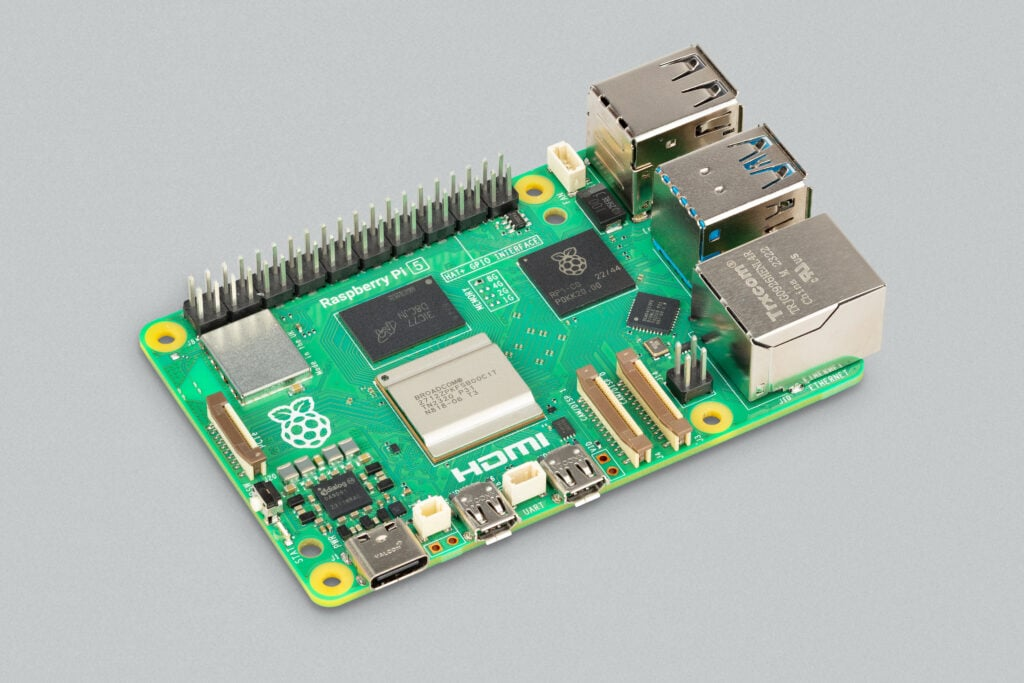
\includegraphics[width=0.6\textwidth]{figures/raspberrypi5.jpg}
    \caption{\textit{RaspberryPI5} \cite{introRaspberrypi5}}
    \label{fig:Raspberrypi5}
\end{figure}

Sendo assim, de forma a cumprir um dos pressupostos referidos anteriormente, surgiu um segundo objectivo que se prende com a eliminação do \acrshort{labview}, o \acrshort{ide} inicialmente proposto. De facto, os preços das diversas versões variam, aproximadamente, entre os 523€ e os 4300€ anuais \cite{labviewpricing}.

No entanto, a eliminação do \acrshort{labview} exigia a implementação de um servidor. De entre as várias opções analisadas, tais como, \textit{FastApi}\footnote{\url{https://fastapi.tiangolo.com/}}, \textit{Django}\footnote{\url{https://www.djangoproject.com/}} ou \textit{Node-RED}\footnote{\url{https://nodered.org/}}, optou-se por implementar o servidor baseado no \textit{Flask}\footnote{\url{https://flask.palletsprojects.com/en/3.0.x/}}. As razões da escolha serão apresentadas na Secção \ref{sec:software}. 

Considerou-se, portanto, que seria uma mais-valia desenvolver um \acrshort{laboratório remoto}, cuja linguagem principal assentaria em \textit{Python}, o servidor em \textit{Flask} e o \textit{interface} com o utilizador desenvolvido em \acrfull{html}. O \gls{RaspberryPI} será responsável pela parte central de controlo dos relés, comunicação com o \acrshort{virtualbench} e como servidor \textit{web}.

Com os objectivos principais definidos na Secção \ref{sec: Objectivos} e com base nos pressupostos referidos anteriormente, estava dado o passo final para o que viria a ser o \acrshort{lare}.

\section{Solução proposta}
\label{sec:solucaoproposta}
Definidas - de uma forma geral - as soluções de \textit{hardware} e \textit{software} - passou-se ao estudo da integração do \acrshort{virtualbench} no \acrshort{lare}, mais especificamente, da integração do \acrshort{virtualbench} com o \gls{RaspberryPI}. 

O \textit{pyVirtualBench} é um \gls{wrapper}\footnote{Este \gls{wrapper} é um \textit{software} de terceiros, suportada e mantida por comunidade de engenheiros e não é diretamente suportado pela \acrshort{ni}.} que permite controlar o \acrshort{virtualbench} através de uma aplicação \textit{Python} \cite{pyvirtualbench}. No entanto, este \gls{wrapper} não é compatível com \textit{Linux}. 
Perante este facto, decidiu-se integrar um \acrshort{pc} no \acrshort{lare} - pormenores da instalação do \textit{driver} no \textit{site} da \acrshort{ni} (\href{https://knowledge.ni.com/KnowledgeArticleDetails?id=kA00Z000000kHUFSA2&l=pt-PT}{\textit{link}}) - sendo que todo o peso computacional passaria para o \acrshort{pc} e o \gls{RaspberryPI} controlaria os relés. 

Na Figura \ref{fig:representaçãogerallare} apresenta-se a representação geral do \acrshort{lare}.

\begin{figure}[hbtp]
    \centering
    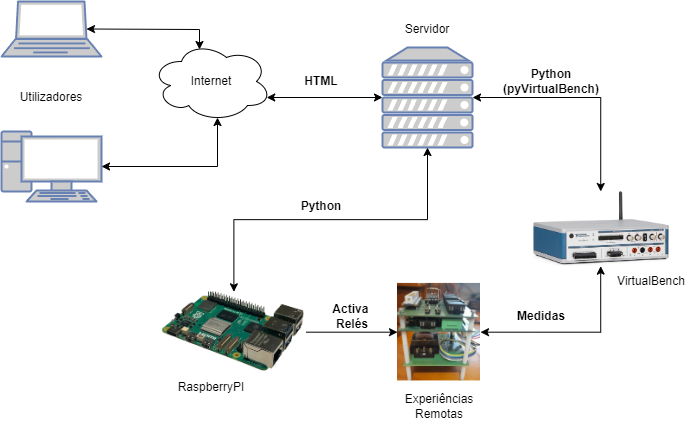
\includegraphics[width=1\textwidth]{figures/arquitectura_ver2.drawio.png}
    \caption{Representação geral do \acrshort{lare}}
    \label{fig:representaçãogerallare}
\end{figure}

No \acrshort{visir} do \acrshort{isep}, estão disponíveis 11 circuitos, como se pode ver na Figura \ref{fig:circuitosvisir}. Os circuitos que compõem o \acrshort{laboratório remoto} tiveram como base (ou ponto de partida) os que estão implementados no \acrshort{isep}. \textbf{Faz sentido? PROF}

\begin{figure}[hbtp]
    \centering
    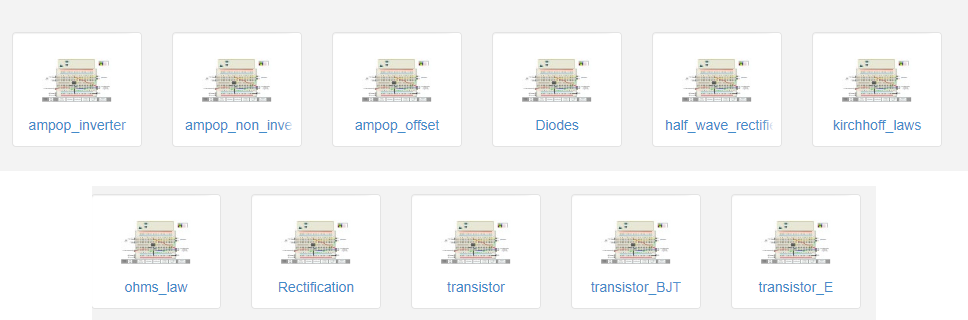
\includegraphics[width=1\textwidth]{figures/visir_ISEP.png}
    \caption{Circuitos \acrshort{visir} - \acrshort{isep}}
    \label{fig:circuitosvisir}
\end{figure}

Sendo assim, os circuitos que compõem o \acrshort{lare} são (\textbf{na implemetação desenvolver um pouco mais sobre as escolhas}):
\begin{itemize}
    \item Lei de Ohm; 
    \item Rectificador de meia onda;
    \item Rectificador de onda completa;
    \item Filtro RC passa-baixo;
    \item Filtro RC passa-alto.
\end{itemize}

\subsection{Matriz LaRE}
Encontradas as soluções de \textit{hardware} e \textit{software}, falta, ainda, uma peça-chave na implementação do \acrshort{laboratório remoto}: a Matriz \acrshort{lare} de relés.

Esta matriz, que inclui os circuitos definidos na Secção \ref{sec:solucaoproposta}, assim como a alimentação e as ligações ao \gls{RaspberryPI}, compõe as 5 experiências.

Esta matriz é composta por 3 placas:
\begin{itemize}
    \item Alimentação:
    \begin{itemize}
        \item Transformador;
        \item Fonte de tensão de \SI{5}{\volt};
    \end{itemize}
    \item Circuito da Lei de Ohm;
    \item Circuitos de Rectificação e filtros:
    \begin{itemize}
        \item Rectificação de meia onda;
        \item Rectificação de onda completa;
        \item Filtro passa-baixo;
        \item filtro passa-alto.
    \end{itemize}
\end{itemize}

A dimensão das placas \gls{pc/104} tem por base os valores descritos no \textit{datasheet} que pode ser encontrado em \url{https://pc104.org/}.

Toda a informação relevante referente à Matriz encontra-se no \textit{datasheet} em anexo. [\textbf{Confirmar as referências e local da aprsentação do datasheet}]

\subsection{Objectivos}
\subsection{Análise de alternativas/razões das opções}
\textbf{Eventualmente já foram abordadas as escolhas do software e hardware no contexto}

\section{Arquitectura}
\begin{figure}[hbtp]
    \centering
    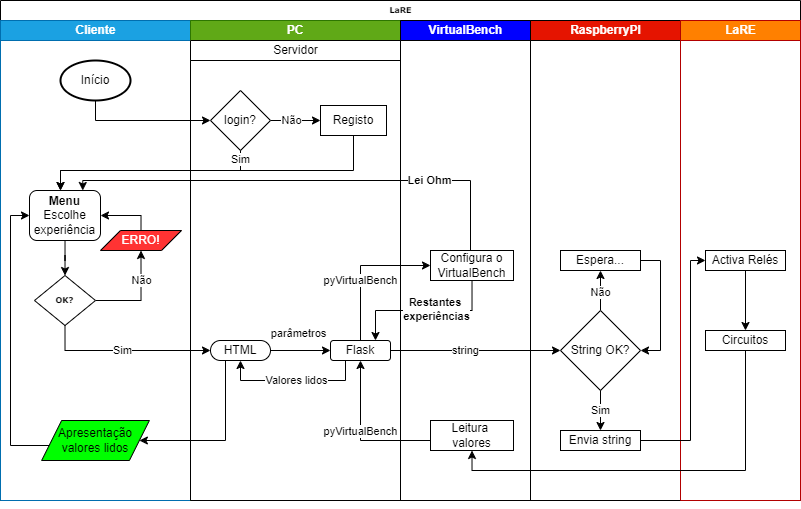
\includegraphics[width=1\textwidth]{figures/Diagrama_SOFTWARE.drawio.png}
    \caption{Arquitectura \acrshort{lare}}
    \label{fig:arquitecturalore}
\end{figure}

Como já vimos na Secção \ref{sec:solucaoproposta} a arquitectura do \acrshort{lare} proposta baseia-se numa estrutura cliente-servidor, suportada ao nível do \textit{hardware} pelo \acrshort{virtualbench}, pelo \gls{RaspberryPI} e um \acrshort{pc} como servidor. 

Ao nível do \textit{software}, o servidor será implementado com base no \textit{Flask}, como será descrito com mais pormenor na Secção \ref{sec:software}. A comunicação entre o servidor e o \acrshort{virtualbench}, entre o servidor e o \gls{RaspberryPI} e o controlo dos relés é feita em \textit{Python}. A \textit{interface} com o utilizador é feita em \acrshort{html}.

A Figura {\ref{fig:arquitecturalore}} apresenta a solução implementada no \acrshort{lare}. De uma forma geral, podemos ver como é realizada a comunicação entre os diferentes dispositivos de \textit{hardware}.

\subsection{Hardware}
\label{sec:hardware}
\subsubsection{VirtualBench}
No contexto desta dissertação o dispositivo sugerido para implementar o \acrshort{lare} foi o \textit{VirtualBench}, modelo VB-8012. Este dispositivo desenvolvido pela \acrshort{ni} integra vários instrumentos e ferramentas de teste, tais como um osciloscópio de sinal misto com análise de protocolo, um gerador de formas de onda, um multímetro digital, uma fonte de alimentação \acrfull{cc} programável e E/S digitais num único dispositivo que se liga a um \acrshort{pc} ou \textit{iPad}, via \acrshort{usb} ou rede sem fios, como se pode ver na Figura \ref{fig:paineltraseiro}. As principais características deste modelo estão descritas na Figura \ref{fig:paineldianteiro} \cite{datasheetVirtualBench}.

A \acrshort{ni} disponibiliza algumas \acrshort{api}s, tais como \acrshort{labview}, ANSI C e Python, esta última não suportada oficialmente.

\begin{figure}
     \centering
     \begin{subfigure}[b]{1\textwidth}
         \centering
         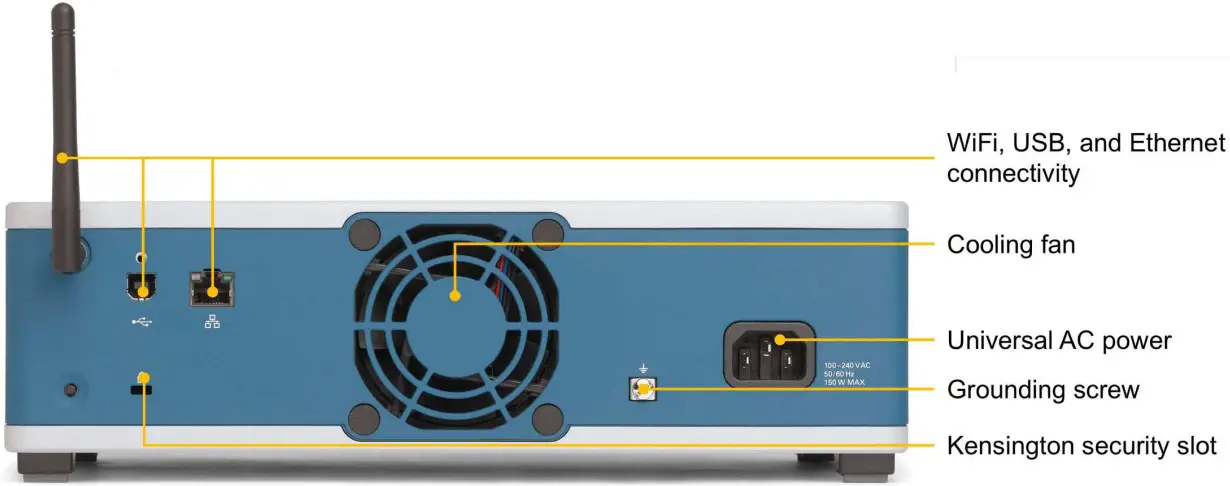
\includegraphics[width=\textwidth]{figures/virtualbench_back-panel.jpg}
         \caption{Painel traseiro  \cite{datasheetVirtualBench}.}
         \label{fig:paineltraseiro}
     \end{subfigure}
     \hfill
     \begin{subfigure}[b]{1\textwidth}
         \centering
         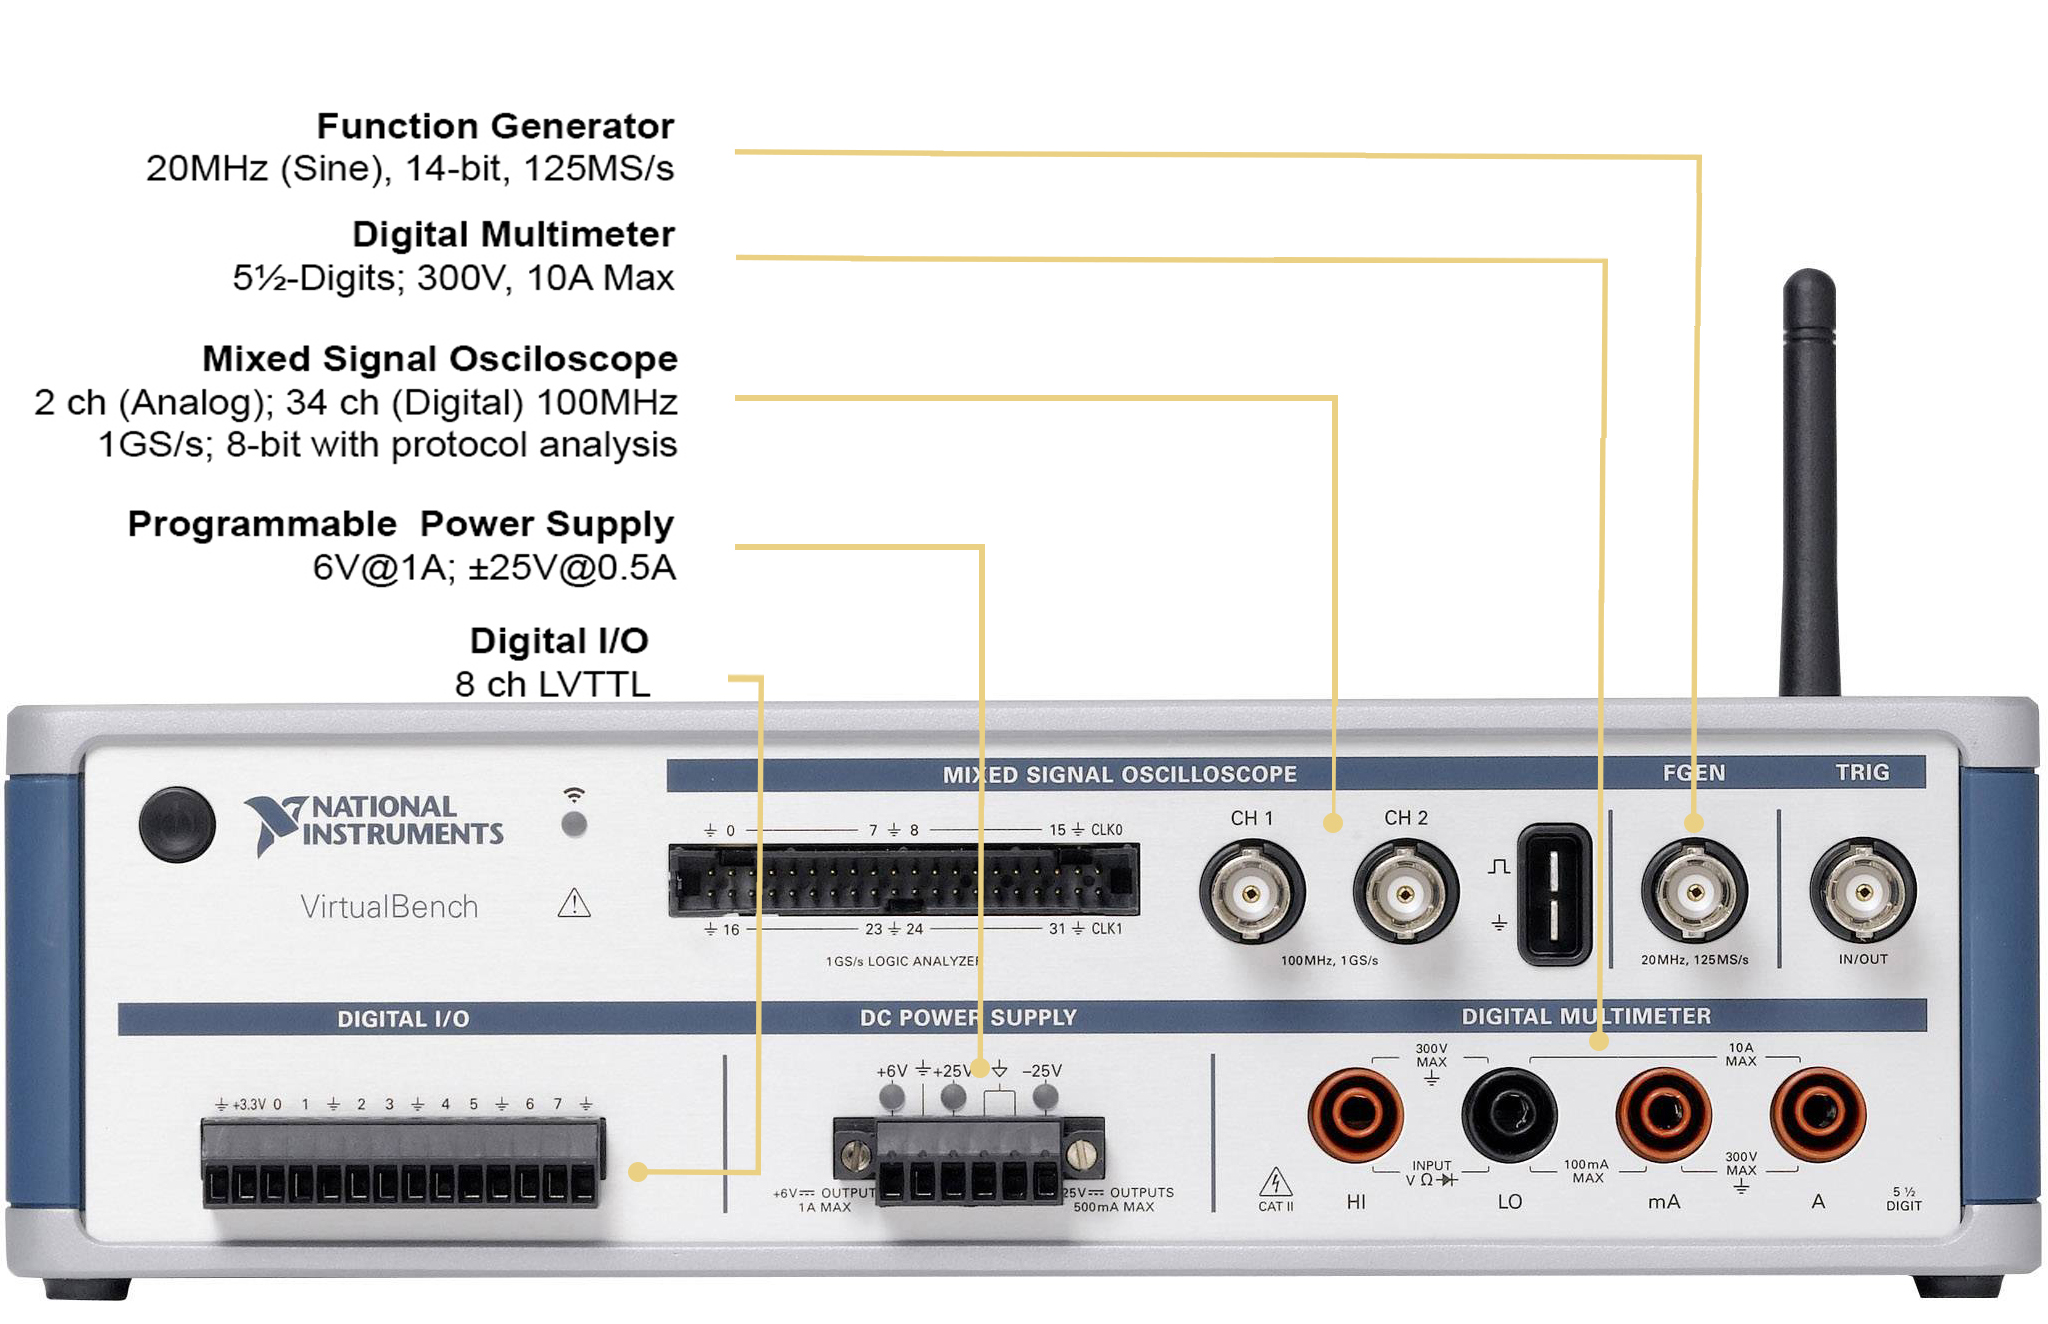
\includegraphics[width=\textwidth]{figures/virtualbench_front-panel.jpg}
         \caption{Painel frontal  \cite{datasheetVirtualBench}.}
         \label{fig:paineldianteiro}
     \end{subfigure}
     \hfill
    \caption{\textit{VirtualBench} VB-8012}
    \label{fig:VB8012}
\end{figure}

Como já foi referido na Secção \ref{sec:solucaoproposta}, o \textit{pyVirtualbench} é uma das formas de controlar o \acrshort{virtualbench}, a outra é através do \textit{software} fornecido e suportado pela \acrshort{ni}.

O \textit{software VirtualBench} é um controlador, que inclui uma aplicação \textit{Windows} que fornece uma apresentação integrada dos cinco instrumentos apresentados no \acrshort{virtualbench}, como pode ser visto na Figuras \ref{fig:interfaceVB} e \ref{fig:leituraohm}. A aplicação também inclui funcionalidades de fluxo de trabalho, como a importação e exportação de configurações de instrumentos e a captura de dados\footnote{\href{https://www.ni.com/en/support/downloads/drivers/download.virtualbench-software.html}{Transferir VirtualBench}}.

\vspace{0.5cm}
\textbf{De referir que o \acrshort{virtualbench} não pode ser controlado pelo \textit{pyVirtualBench} e pelo \textit{software} simultaneamente}.
\vspace{0.5cm}

\begin{figure}
     \centering
     \begin{subfigure}[b]{1\textwidth}
         \centering
         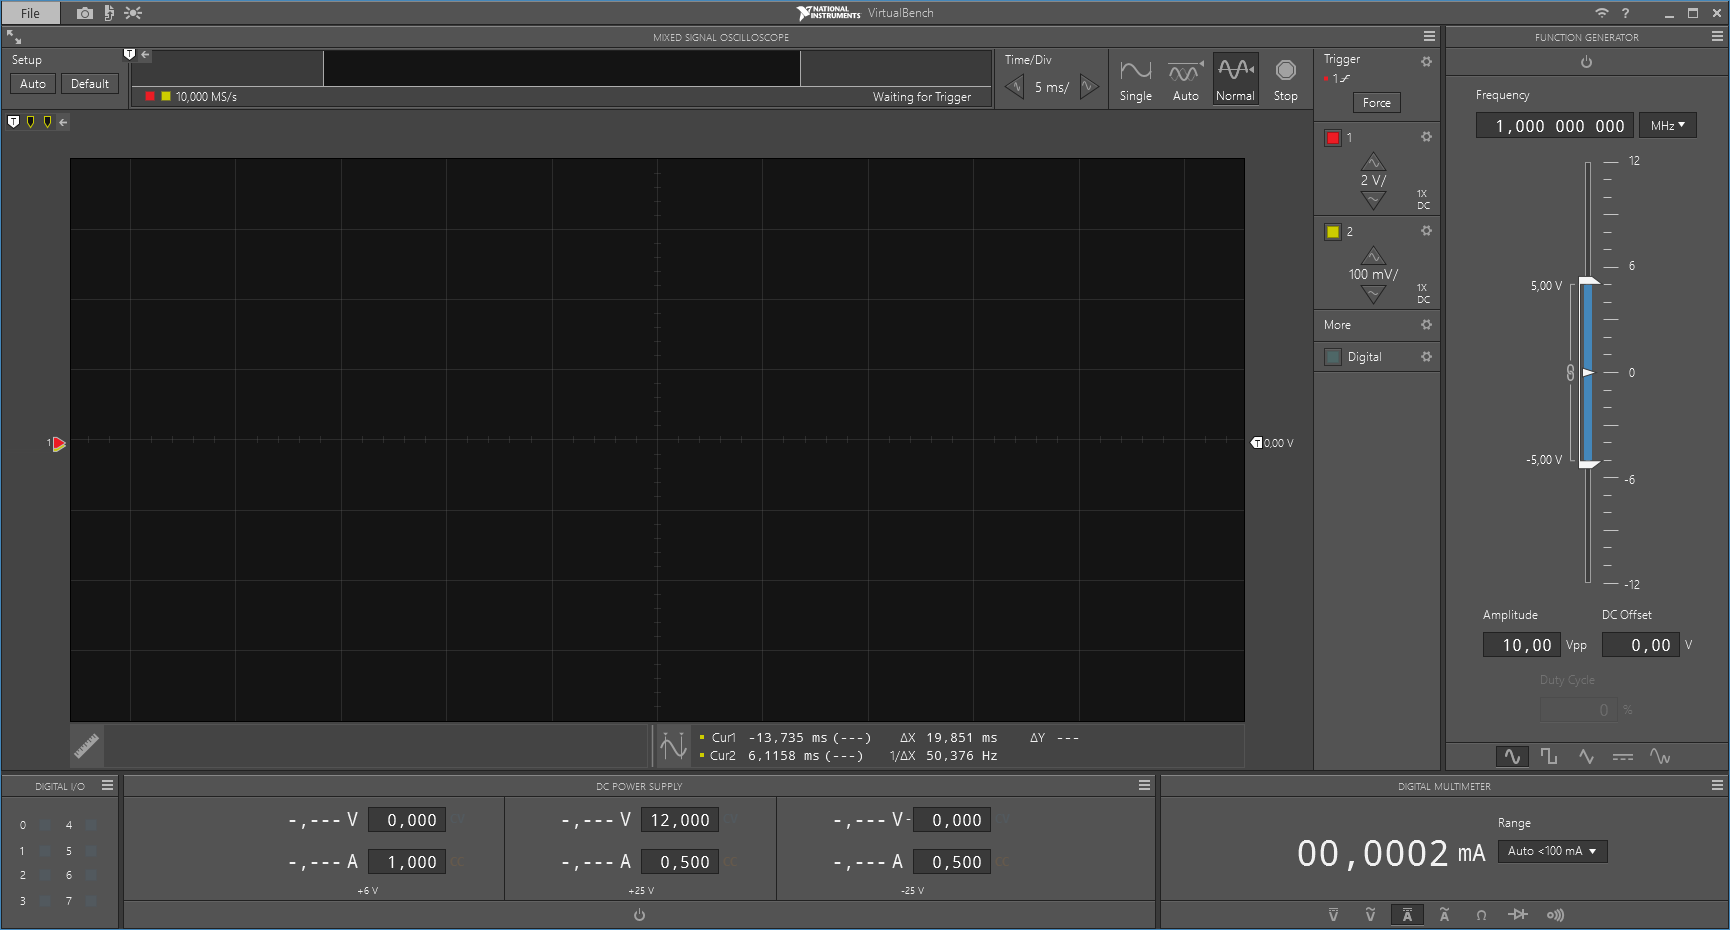
\includegraphics[width=\textwidth]{figures/VB8012-Desktop.png}
         \caption{\textit{Interface} do \acrshort{virtualbench}}
         \label{fig:interfaceVB}
     \end{subfigure}
     \hfill
     \begin{subfigure}[b]{1\textwidth}
         \centering
         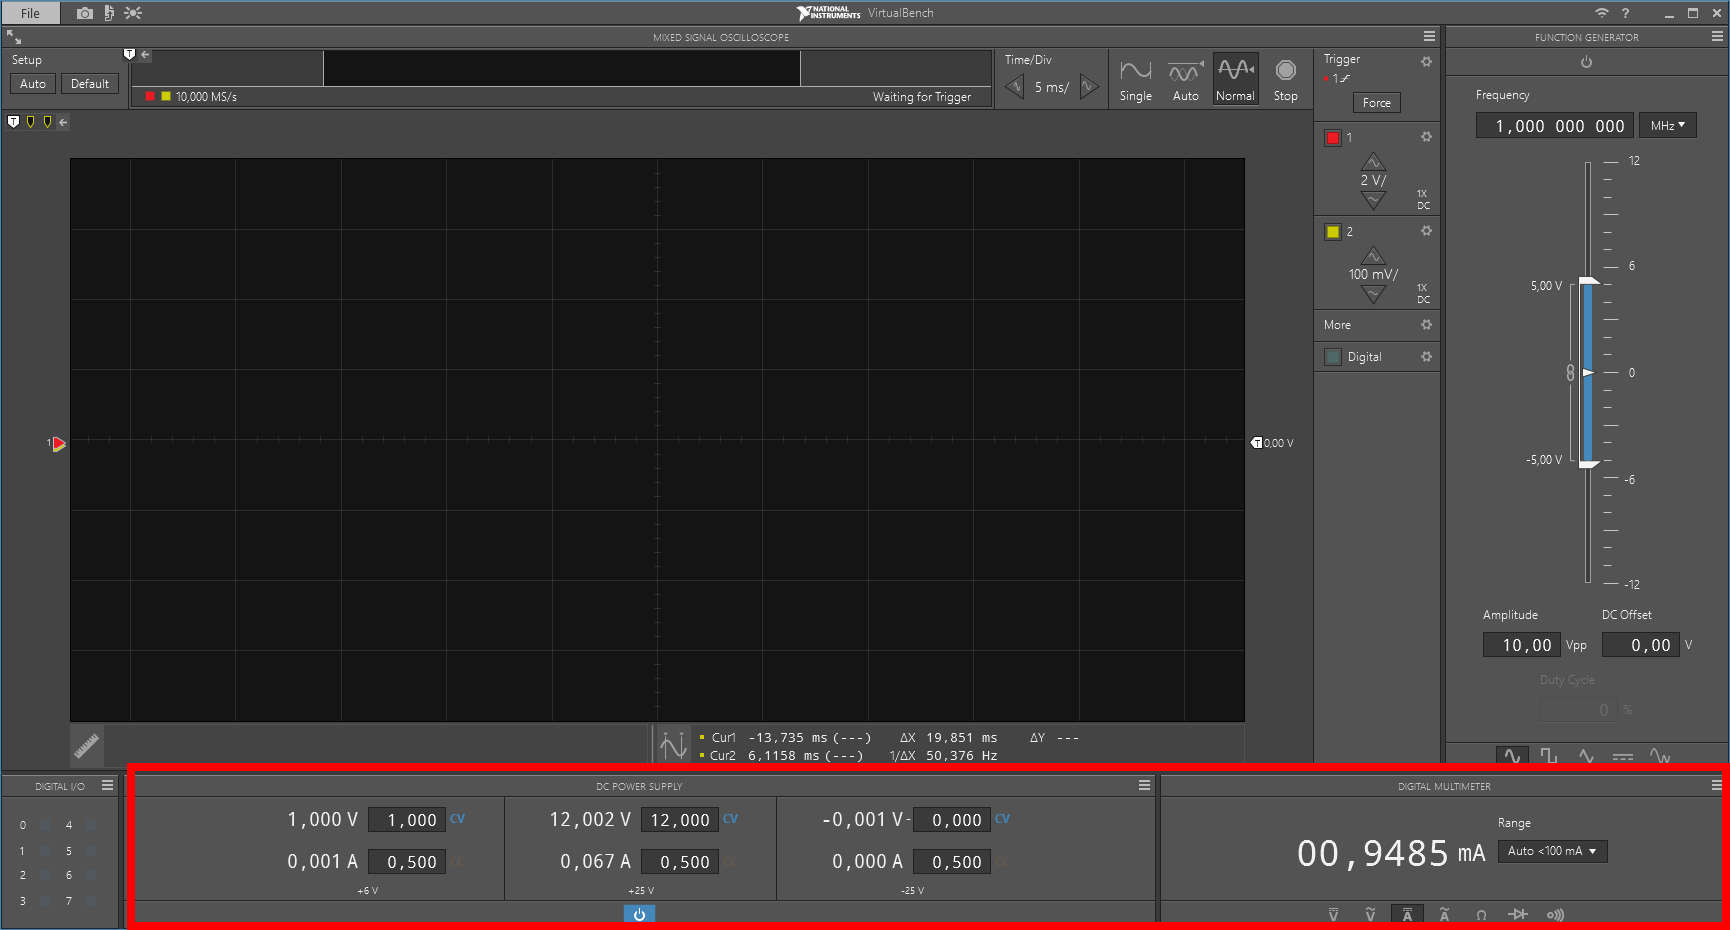
\includegraphics[width=\textwidth]{figures/VB8012-OHM_Exemplo.png}
         \caption{Utilização do multímetro digital no \acrshort{virtualbench}}  
         \label{fig:leituraohm}
     \end{subfigure}
     \hfill
    \caption{\textit{VirtualBench}}
    \label{fig:VB_OHM_Exemplo}
\end{figure}

\subsubsection{RaspberryPI}
Como já foi referido na Secção \ref{sec:contextualização}, a ideia inicial passava por utilizar o \gls{RaspberryPI} como servidor e como controlador dos relés, no fundo desempenhando as funções de \acrshort{rlms}.

No entanto, o \textit{pyVirtualBench} é incompatível com o \gls{RaspberryPI}. A decisão de o manter como controlador dos relés prendeu-se com o facto de, futuramente, poder haver espaço para uma evolução ao nível da compatibilidade no \textit{pyVirtualBench}.

Em contexto de laboratório estavam disponíveis os modelos PI2 e PI3, algo desactualizados. O PI3 já se mostrou lento nos primeiros testes e, por isso, optou-se pela última versão do \textit{RaspberryPI}\footnote{Doravante, sempre que for referido \textit{RaspberryPI}, subentende-se a versão 5.}.

As principais diferenças de \textit{hardware} entre a versão 5 e a 4B estão representadas na Tabela \ref{Table:diferencasPI4PI5}. Estas melhorias acarretam um maior consumo de energia e, por isso, é recomendado o uso de arrefecimento. Na Figura \ref{fig:pi5dissipador} está representado o \gls{RaspberryPI} usado no \acrshort{lare}.

\textbf{Referência aos pinos no datasheet?}

\begin{figure}[hbtp]
    \centering
    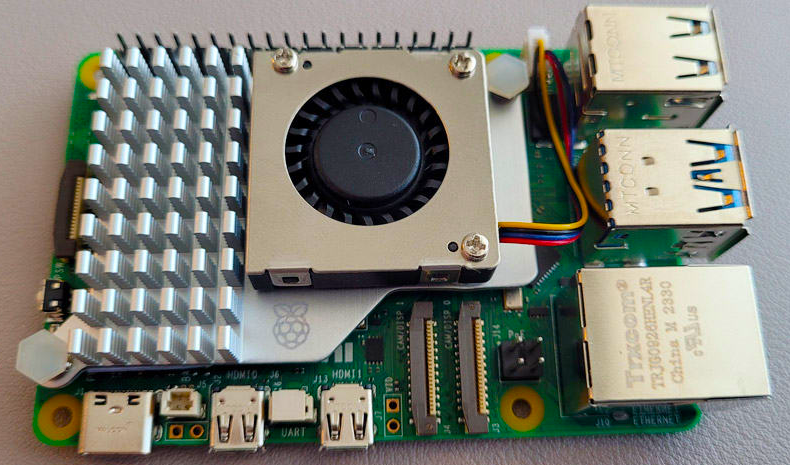
\includegraphics[width=1\textwidth]{figures/pi5_dissipador.png}
    \caption{\textit{Raspberry PI5} com dissipador activo utilizado no \acrshort{lare}}
    \label{fig:pi5dissipador}
\end{figure}

\begin{table}[htb]
\centering
\caption{Raspberry PI4 \textit{vs Raspberry PI5 - principais diferenças} \cite{Raspberrypi5}}
\label{Table:diferencasPI4PI5}
\begin{tabular}{ll}
\toprule
Raspberry PI4 & Raspberry PI5 \\
\midrule
\SI{1.8}{\giga\hertz} & \SI{2.4}{\giga\hertz} \\
\midrule
VideoCore VI @ \SI{500}{\mega\hertz}, Vulkan 1.0 & VideoCore VII @ \SI{800}{\mega\hertz}, Vulkan 1.2 \\
\midrule
LPDDR4-3200 SDRAM até \SI{8}{\giga\byte} & LPDDR4X-4267 SDRAM \SI{4}{\giga\byte}/\SI{8}{\giga\hertz} \\
\midrule
\SI{5}{\volt}/\SI{3}{\ampere} via USB-C (\SI{15}{\watt}) & \SI{5}{\volt}/\SI{5}{\ampere} via USB-C (\SI{27}{\watt})\\
\bottomrule
\end{tabular}
\end{table}

\subsubsection{Relés}
Os relés utilizados estavam disponíveis em contexto laboratorial e são em tudo idênticos aos que se encontram montados no \acrshort{visir}  do \acrshort{isep}.

No \acrshort{lare} foram usados dois tipos de relés - simples, \acrfull{spst} e duplos, \acrfull{dpst}, como se pode ver na Figura \ref {fig:reles}.

Os modelos utilizados foram ambos da \textit{Comus}: relé \acrshort{spst}, ref. 3570-1331-123 e relé \acrshort{dpst}, ref. 3572-1220-123. As características mais importantes encontram-se descritas no \textit{datasheet} anexo a este documento. \textbf{Ver a referência ao datasheet}. Os dois primeiros quartetos indicam a série do relé e os três números indicam a tensão da bobine e a presença, ou não, do díodo de ``roda livre''. No caso dos relés usados, a tensão da bobine é de \SI{12}{\volt} e o díodo está ligado entre os pinos 2(+) e 6(-) \cite{DryRelay}. Tentou-se, sempre que possível, utilizar os relés \acrshort{spst} no comando das fontes e aparelhos de medida e os relés \acrshort{dpst} no controlo dos componentes. Serão devidamente referidos os casos em que isso não foi possível, por indisponibilidade dos componentes.

\begin{figure}[hbtp]
    \centering
    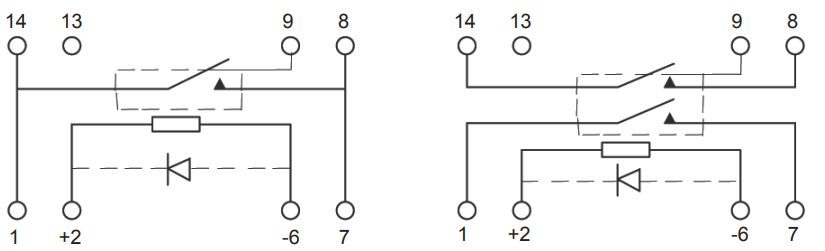
\includegraphics[width=1\textwidth]{figures/reles.png}
    \caption{\textit{Relés \acrshort{spst} e \acrshort{dpst}} \cite{DryRelay}}
    \label{fig:reles}
\end{figure}

 Segundo a informação técnica disponibilizada em \cite{Raspberrytech}, a tensão de funcionamento dos \acrfull{gpio}s, quer estejam configurados como entrada ou saída, é de \SI{3.3}{\volt}, sendo que a máxima corrente por cada \acrshort{gpio} é de \SI{16}{\mA}. No caso extremo de todas os 17 \acrshort{gpio}s estarem activos ao mesmo tempo, a corrente total seria de \SI{272}{\mA}. Nesta situação, a fonte de \SI{3.3}{\volt} colapsava. 
 Por isso, para que o RaspberryPI possa comandar os relés com segurança, é necessário o uso de \textit{drivers} que consigam fornecer a tensão e corrente necessária para o efeito.
 
 \subsubsection{\textit{Driver} de Relés}
 O circuito integrado ULN2003A é um \textit{driver} muito usado para controlar relés. Além disso e mais uma vez, estava disponível em contexto laboratorial.
Tipicamente, este \textit{driver} é usado em conjunto com micro-controladores ou \gls{RaspberryPI} no comando de cargas indutivas, como motores, bobines e relés. 

Os ULN2003A possuem sete pares de transístores NPN, em configuração \textit{Darlington}, que apresentam saídas de alta tensão com díodos \textit{clamp} de cátodo comum para comutação de cargas indutivas \cite{ULN2003}, como se  representa esquematicamente na Figura \ref{fig:2003blocos}.

\begin{figure}[hbtp]
    \centering
    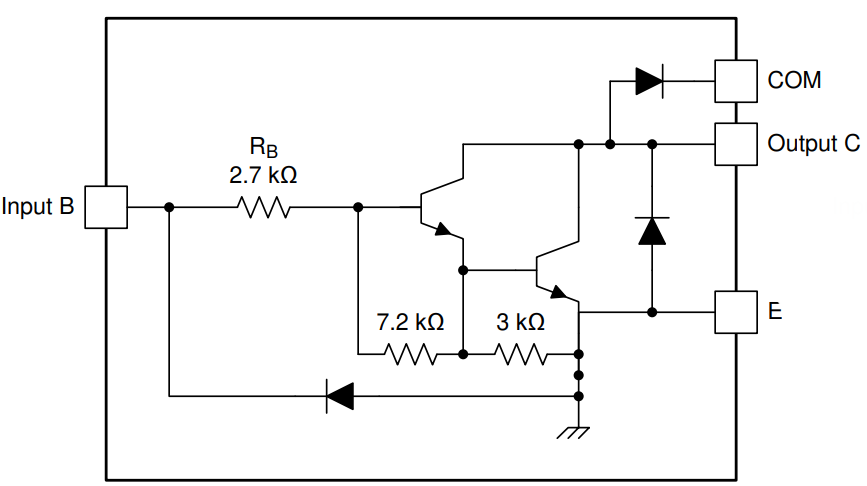
\includegraphics[width=1\textwidth]{figures/2003A_Darling.png}
    \caption{Diagrama de blocos ULN2003A \cite{ULN2003}}
    \label{fig:2003blocos}
\end{figure}

A corrente de colector de saída (única) é de \SI{500}{\mA} e a corrente de entrada, para uma tensão de entrada de \SI{3.85}{\volt}, é \SI{0.93}{\mA} \cite{ULN2003}.

Pela análise dos esquemas \textbf{DATASHEET - REFERÊNCIA} verifica-se que os \acrshort{gpio}s disponíveis no \gls{RaspberryPI} - 17 no total - não são suficientes para comandar os relés do \acrshort{lare}. Ao todo são utilizados 21 relés, o que corresponderia a 21 saídas. A placa correspondente à experiência da Lei de Ohm, possui 8 relés. No caso da placa correspondente às experiências dos circuitos de rectificadores e filtros, o número de relés para efectuar as experiências é de 13. Falta adicionar os 10 \acrshort{gpio}s necessários para o controlo da transmissão das tramas de \textit{bits} \footnote{Este procedimento será abordado com mais \textbf{rigor, explicado melhor, blá, blá, nas secções seguintes - COLOCAR REFERÊNCIA}}.

Sendo assim, houve a necessidade de criar uma solução que permitisse comandar os relés, já que o \gls{RaspberryPI} não possui \acrshort{gpio}s suficientes.

\subsubsection{Registo de deslocamento}
O uso de registos de deslocamento foi a solução encontrada de forma a ultrapassar o problema da falta de \acrshort{gpio}s. 

O SN74HC595 é um circuito integrado comum e bastante utilizado que contém um registo de deslocamento de 8 bits com saídas \textit{3-State}, do tipo \acrfull{sipo}, que alimenta um registo de armazenamento do tipo D, também de 8 \textit{bits} e com saídas paralelas \textit{3-State}. O relógio é independente para o registo de deslocamento e armazenamento. A potência consumida é muito baixa, assim como a corrente de entrada \cite{SN74HC595}.

Neste caso, os \textit{bits} são enviados um-a-um, armazenados no registo e depois enviados para a saída. A Figura \ref{fig:SN74HC595blocos} representa o diagrama de blocos do SN74HC595 e a Tabela \ref{Table:funcSN74HC595} representa os modos de funcionamento.

\begin{figure}[hbtp]
    \centering
    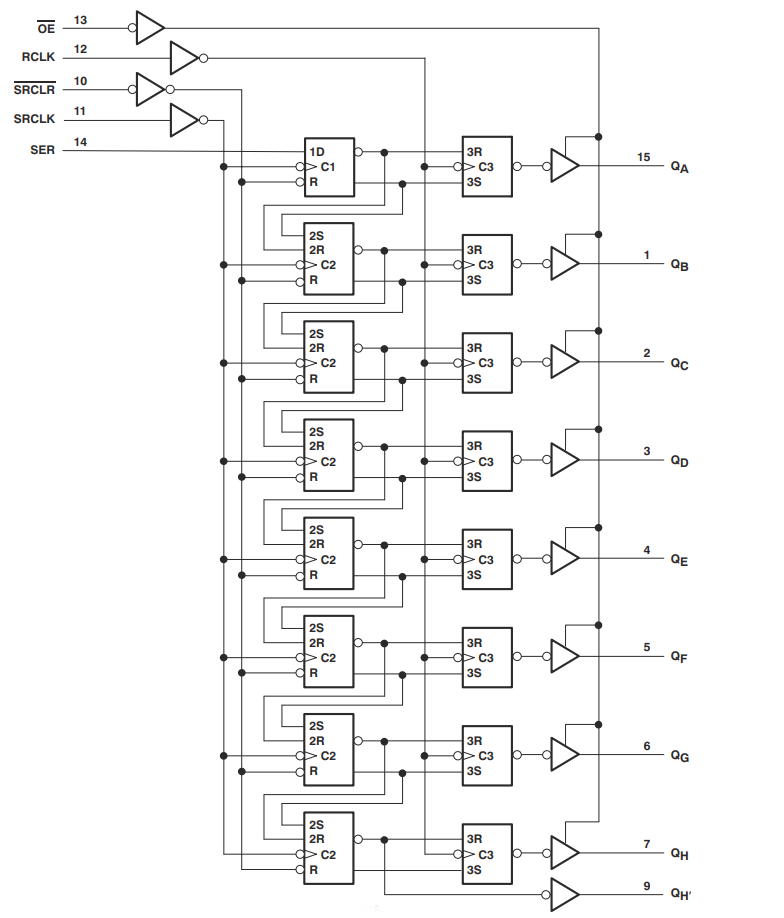
\includegraphics[width=1\textwidth]{figures/SR_blocos.png}
    \caption{Diagrama de blocos SN74HC595 \cite{SN74HC595}}
    \label{fig:SN74HC595blocos}
\end{figure}h

Na transmissão das tramas optou-se por dividir as duas: envio de 8 \textit{bits} na experiência da Lei de Ohm e envio de 13 \textit{bits} nas experiências de rectificadores e filtros. Como se pode ver na Tabela \ref{Table:funcSN74HC595}, são precisos 5 \acrshort{gpio}s (ou 5 saídas) para controlar o envio de uma trama, portanto, para realizar o comando dos relés do \acrshort{lare}, são/serão necessários 10 \acrshort{gpio}s.
Nos capítulos seguintes - \textbf{COLOCAR A REFERÊNCIA} - é explicado com mais pormenor o processo de envio. As implicações ao nível do \textit{software} de programação são mínimas e ao nível do \textit{hardware} estão dentro dos limites de número de \acrshort{gpio}s do \gls{RaspberryPI}.

\begin{table}[htb]
\caption{Modos de funcionamento do SN74HC595 \cite{SN74HC595}}
\label{Table:funcSN74HC595}
\resizebox{\textwidth}{!}{%
\begin{tabular}{cccccl}
\toprule
\multicolumn{5}{c}{Entradas} & \multicolumn{1}{c}{\multirow{3}{*}{Função}} \\
\cline {1-5}
\multicolumn{5}{l}{} &
  \multicolumn{1}{c}{} \\
  \multicolumn{1}{l}{SER} &
  \multicolumn{1}{l}{SRCLK} &
  \multicolumn{1}{l}{$\overline{SRCLR}$} &
  \multicolumn{1}{l}{RCLK} &
  \multicolumn{1}{l}{$\overline{OE}$} & 
  \multicolumn{1}{c}{} \\
  \midrule
X    & X   & X   & X   & H   & Saídas $Q_A$ – $Q_H$ estão desabilitadas. \\
\midrule
X    & X   & X   & X   & L   & Saídas $Q_A$ – $Q_H$ estão habilitadas. \\
\midrule
X    & X   & L   & X   & X   & Registo de deslocamento é limpo. \\
\midrule
L &
 $\uparrow$  &
  H &
  X &
  X &
  \begin{tabular}[c]{@{}l@{}} Primeiro passo do registo de deslocamento vai a ``0''. \\ Passo seguinte armazena os dados do estado anterior, respectivamente. \end{tabular} \\
  \midrule
H &
 $\uparrow$  &
  H &
  X &
  X &
  \begin{tabular}[c]{@{}l@{}}Primeiro passo do registo de deslocamento vai a ``1''. \\ Passo seguinte armazena os dados do estado anterior, respectivamente. \end{tabular} \\
  \midrule
X    & X   & X   &  $\uparrow$   & X   & Os dados do registo de deslocamento são armazenados no registo.\\
\bottomrule
\end{tabular}%
}
\end{table}

\textbf{No datasheet em tal sítio está representada informação complementar respeitante ao ULN2003A e 74595}

\subsubsection{Outras coisas | Vários}
\textbf{Acho que nada tenho a referir, pelo menos que me lembre}
\subsection{Software}
\label{sec:software}
O \textit{software} do \acrshort{lare} foi dividido em duas grandes grupos/partes/secções(riscar o que não interessa): \textit{Back-end} e \textit{Front-end}.

Por \textit{Back-end} pode entender-se toda a programação e os processos a correr em segundo plano, que sustentam o funcionamento do \acrshort{lare}, incluindo servidor, \acrshort{api}s ou base de dados \cite{FrontbackEnd}. Existe uma grande variedade de linguagens de programação, \textit{frameworks} e ferramentas para realizar a gestão do \textit{Back-end}. Na implementação do \acrshort{lare}, utilizou-se o \textit{Python} como linguagem de programação e o \textit{Flask} como \textit{Framework}.

Já o \textit{Front-end} gere as partes dos \textit{sites} e das aplicações que os utilizadores veem e com as quais interagem para realizar determinadas tarefas. As linguagens utilizadas na implementação do \textit{Front-end} para o \acrshort{lare} foram o \acrshort{html}, \acrfull{css} e \textit{JavaScript}. Enquanto o \acrshort{html} é a ``espinha dorsal'' estrutural de um \textit{site}, o \acrshort{css} lida com a aparência personalizada que define o estilo dos elementos visuais e o JavaScript afecta a forma como os elementos da página se movimentam \cite{FrontbackEnd}.

De uma forma resumida, o desenvolvimento de \textit{Front-end} refere-se ao lado do cliente (aspeto de uma página \textit{Web}) e o desenvolvimento de \textit{Back-end} refere-se ao lado do servidor (funcionamento de uma página \textit{Web}).

\subsubsection{\textit{Back-End}}
\paragraph{\textit{Python}}
A opção por esta linguagem deveu-se a uma série de factores que começaram com a vontade pessoal de desenvolver e evoluir ao nível do conhecimento em \textit{Python}. Além disso, e como já foi referido no Capítulo \textbf{VER REFERÊNCIA}, o comando e configuração do \acrshort{virtualbench} é feito através do \textit{pyVirtualBench}. 

O \textit{Python} é uma linguagem poderosa e fácil de aprender. Possui estruturas de dados de alto nível eficientes e uma abordagem simples, mas eficaz à programação orientada para objectos \cite{ThePython}. Apresenta, também, uma série de vantagens que se enquadram nos objectivos do desenvolvimento e implementação do \acrshort{lare} \cite{pythonvantagens}:
\begin{itemize}
    \item Curva suave de aprendizagem;
    \item Quantidade e variedade das bibliotecas;
    \item Portabilidade;
    \item Flexibilidade;
    \item Robustez;
    \item Suporte da comunidade.
\end{itemize}

Como desvantagens há a referir que, comparado com outras linguagens, o \textit{Python} é mais lento em termos de execução, já que é um tipo de linguagem de alto-nível, não é adaptado para aplicações móveis e consome mais recursos \cite{pythonvantagens} \cite{5MainDispython}.

Ainda assim, segundo a \textit{\href{https://spectrum.ieee.org/the-top-programming-languages-2023}{\textit{IEEE Spectrum}}} o \textit{Python} foi considerada a linguagem mais popular em 2023.

\paragraph{\textit{Flask}}
O \textit{Flask} é uma \textit{framework} leve e flexível para \textit{Python} que segue a filosofia \textit{UNIX} de ``fazer uma coisa bem feita''. A escolha do \textit{Flask} deveu-se, essencialmente, à facilidade de integração com o \textit{Python}, sendo uma das \textit{frameworks} mais populares em \textit{Python} \cite{Flask}. É uma \textit{framework} de aplicações \acrfull{wsgi} que descreve a forma como um servidor \textit{Web} comunica com aplicações \textit{Web} e como essas aplicações podem ser encadeadas para processar um pedido \cite{wsgi}. Depende, ainda do  \textit{Jinja}, que é um motor de criação de modelos que permite escrever código semelhante à sintaxe do \textit{Python}, de forma a renderizar o documento final \cite{Jinja}.

Tal como foi referido na Secção \ref{sec:contextualização}, foram ainda analisadas várias opções, incluindo a \textit{Django}, outra \textit{framework} bastante popular. Em \cite{Djangovsflask} e \cite{FlaskvsDjango}, por exemplo, é feita uma comparação exaustiva entre as duas \textit{frameworks}, não havendo uma decisão final sobre qual a melhor, mas sim sobre qual a que melhor se adapta às necessidades de implementação e desenvolvimento dos projectos. 

No entanto, o \textit{Flask} foi concebido para tornar a iniciação rápida e fácil, com a capacidade de evoluir até aplicações mais complexas, sendo mais adapatado a pequenos projectos. 

Pelas razões referidas anteriormente, assim como a análise feita aos prós e contras, considerou-se que tanto o \textit{Python} como o \textit{Flask} são as linguagens que melhor se enquadram e adaptam aos objectivos propostos para o \acrshort{lare}.

\subsection{Front-End}
\subsubsection{\textit{Webpage}}
Como já foi referido na Secção \ref{sec:software}, o \textit{Front-end} diz respeito ao aspecto gráfico das páginas \textit{Web} e pretende-se que a prioridade na construção da página seja a simplicidade.

A escolha do desenvolvimento da página recaiu no \acrshort{html}, \acrshort{css} e (pontualmente - \textbf{REVER}) \textit{JavaScript}.

O \acrshort{html} é a linguagem de marcação \textit{standard}, usada para definir a estrutura do seu conteúdo e consiste numa série de elementos usados para delimitar ou agrupar diferentes partes do conteúdo. As \textit{tags} podem transformar uma palavra ou imagem num \textit{hiperlink}, podem colocar palavras em itálico, podem aumentar ou diminuir a fonte, etc. etc. \cite{HTMLbasics}.

A folha de estilos \acrshort{css} é o código usado para dar estilo à página. Assim como o \acrshort{html}, o \acrshort{css} não é, realmente, uma linguagem de programação. Também não é uma linguagem de marcação — é uma linguagem de folhas de estilos. Isso significa que o \acrshort{css} permite aplicar estilos seletivamente a elementos em documentos \acrshort{html}.

Já o \textit{JavaScript} é uma linguagem de programação utilizada principalmente para \textit{scripts} dinâmicos do lado do cliente em páginas \textit{web}, podendo também ser utilizada no lado do servidor. É também utilizado no navegador, permitindo que os conteúdos das páginas sejam manipulados através de uma \acrshort{api} \acrfull{dom} ou através de \acrfull{ajax} \cite{HTMLbasics}.